\section{Training}

Training a neural network involves learning a set of parameters, such as weights $\mathbf{w}$, that allow the model $y(x_n|\mathbf{w})$ approximate the target $t_n$ as closely as possible, given a training set $\mathcal{D}=\left\{\left\langle x_1,t_1 \right\rangle,\dots,\left\langle x_N,t_N\right\rangle\right\}$ we want to find model parameters such that for new data $y_n(x_n|\theta)\sim t_n$.
This process can be viewed as finding parameters that generalize well to new data, such that $g(x_n|\mathbf{w})\sim t_n$. 

In regression and classification tasks, this goal is typically achieved by minimizing the error between the predicted outputs and the true labels. 
For a neural network, the error is often represented as the Sum of Squared Errors (SSE):
\[E(\mathbf{w})_{\text{SSE}}=\sum_n^N\left(t_n-g(x_n|\mathbf{w})\right)^2\]
Here, the SSE represents the error function, and for a feedforward neural network, this error is a non-linear function of the weights, making the optimization process more challenging.

\subsection{Nonlinear optimization}
To minimize a generic error function $J(\mathbf{w})$, we rely on optimization techniques.
The goal is to find the weights $\mathbf{w}$ that minimize the error by solving:
\[\dfrac{\partial J(\mathbf{w})}{\partial \mathbf{w}}=0\]
However, for neural networks, closed-form solutions are generally not available due to the non-linearity of the model. 
Instead, we employ iterative methods like gradient descent, which adjusts the weights incrementally in the direction that reduces the error.
The steps for gradient descent are as follows:
\begin{enumerate}
    \item Initialize the weights $\mathbf{w}$ to small random values.
    \item Iterate until convergence: 
        \[w^{k+1}=w^k-\eta\dfrac{\partial J(\mathbf{w})}{\partial \mathbf{w}}\Bigg|_{w^k}\]
        Here, $\eta$ is the learning rate, controlling the step size in each iteration. 
\end{enumerate}
In cases where the error function has multiple local minima, the final solution depends on the initial starting point. 
To address this, we can introduce a momentum term that helps the optimization process avoid being trapped in local minima:
\[w^{k+1}=w^k-\eta\dfrac{\partial E(\mathbf{w})}{\partial \mathbf{w}}\Bigg|_{w^k}-\alpha\dfrac{\partial E(\mathbf{w})}{\partial \mathbf{w}}\Bigg|_{w^k}\]
Here, $\alpha$ represents the momentum coefficient, which encourages the optimization to keep moving in the same direction, effectively smoothing out oscillations and escaping shallow local minima.

\paragraph*{Multiple restarts}
To improve the likelihood of finding the global minimum, especially in complex non-convex error surfaces, multiple restarts of the optimization from different random initializations can be used. 
This increases the chances of converging to a better solution by exploring various regions of the parameter space.

\subsection{Gradient descent}
\begin{example}
    Consider the following feed-forward neural network:
    \begin{figure}[H]
        \centering
        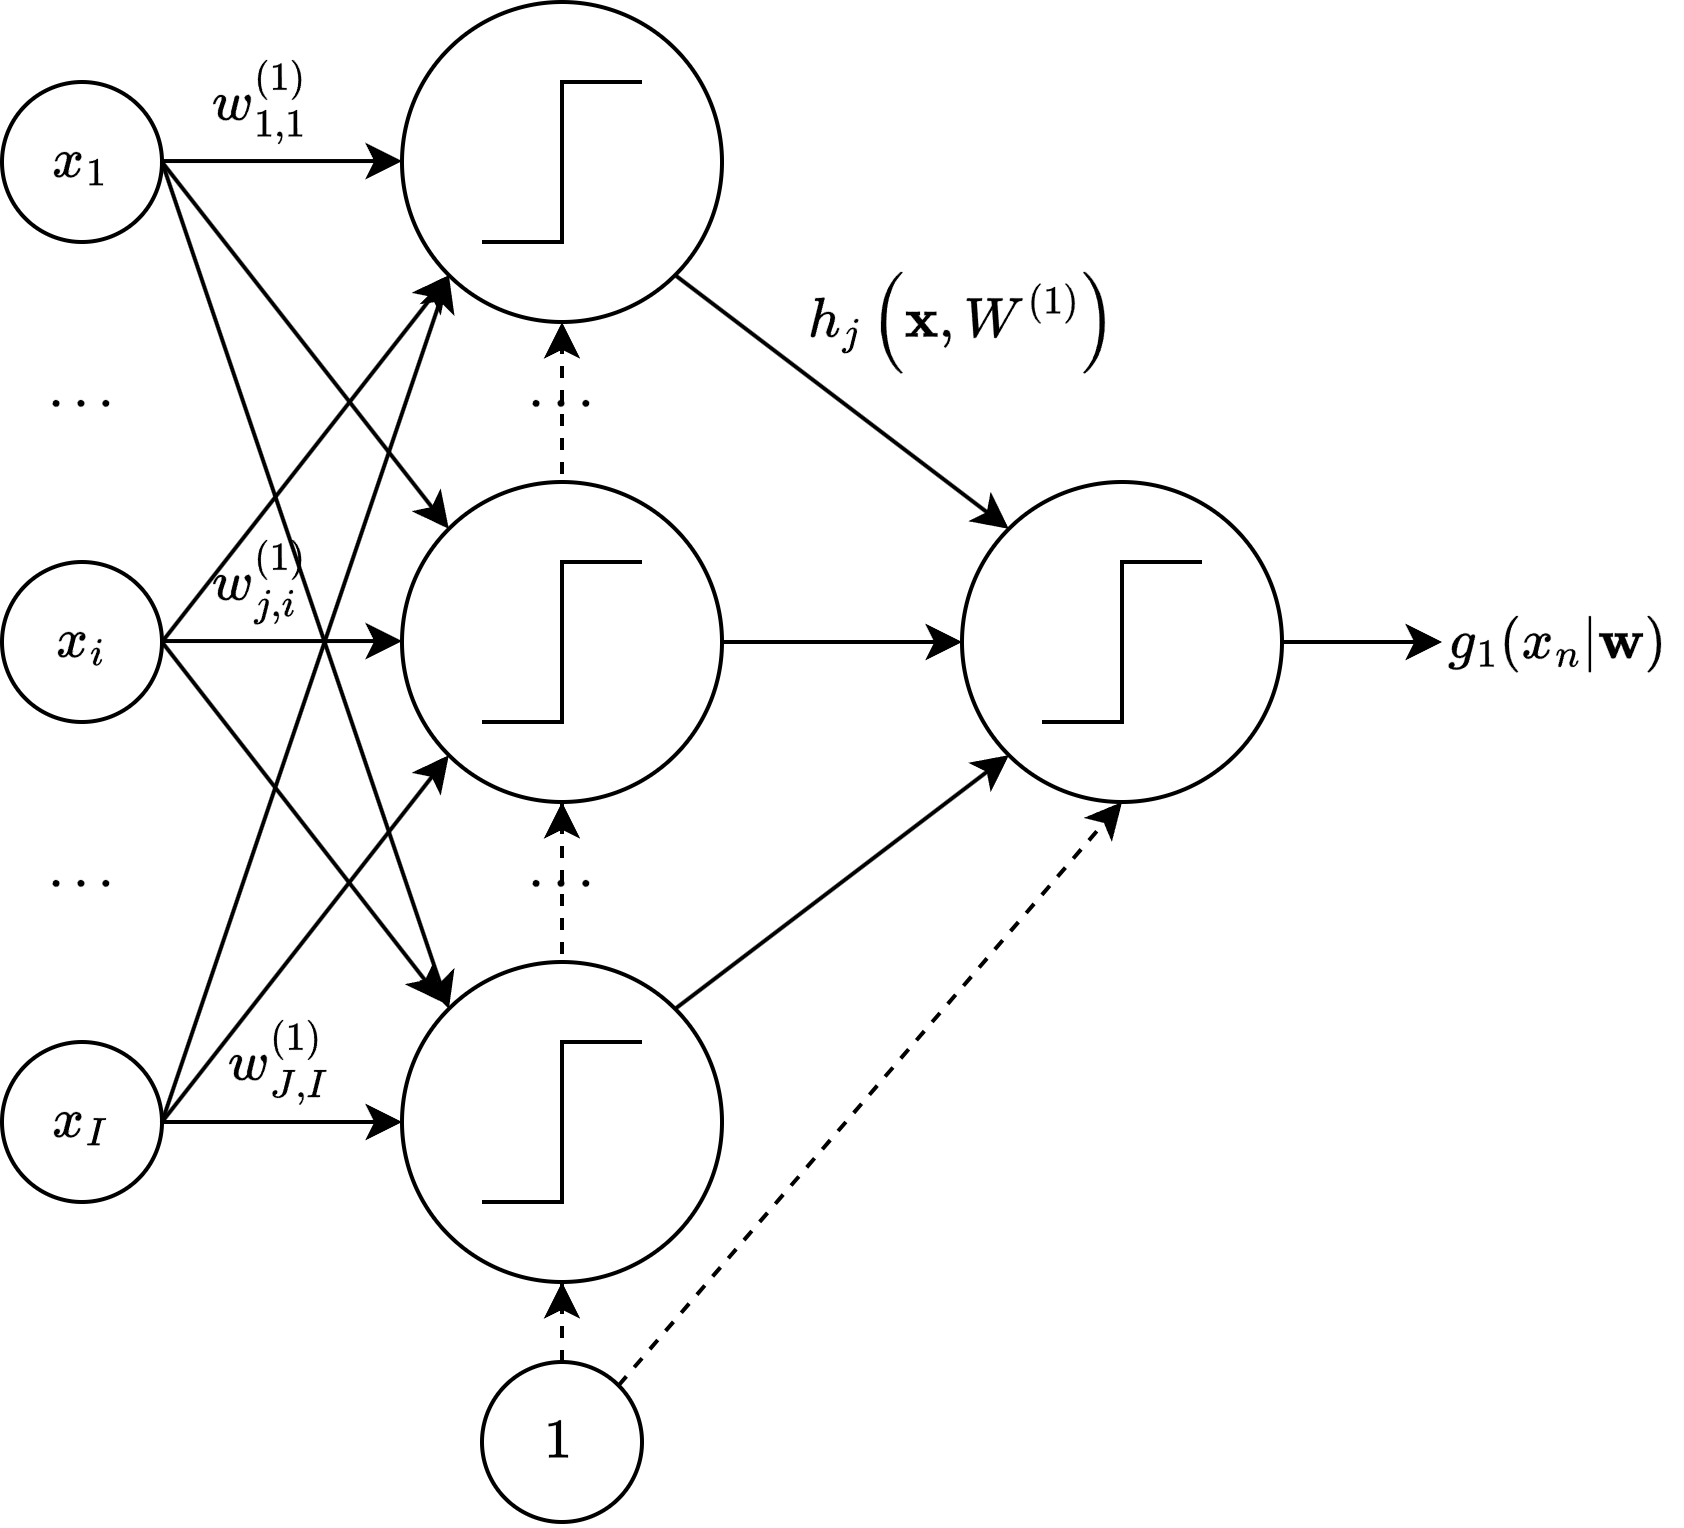
\includegraphics[width=0.60\linewidth]{images/ffnn1.png}
    \end{figure}
    The output of the network is defined as:
    \[g_1(x_n|\mathbf{w})=g_1\left(\sum_{j=0}^Jw_{1,j}^{(2)}h_j\left(\sum_{i=0}^Iw_{j,i}^{(1)}x_{i,n}\right)\right)\]
    Here, $h_j$ represents the activation function of the hidden neurons, and $w_{i,j}^{(1)}$ and $w_{i,j}^{(2)}$ are the weights of the first and second layers, respectively.

    We aim to minimize the sum of squared errors (SSE) between the predicted output and the target values:
    \[E(\mathbf{w})=\sum_{n=1}^N\left(t_n-g_1(x_n|\mathbf{w})\right)^2\]

    Let's compute the weight update for $w_{3,5}^{(1)}$ using gradient descent. 
    This weight corresponds to the connection between the 5th input and the 3rd hidden neuron.
    After calculating the derivative of the error function with respect to $w_{3,5}^{(1)}$, we obtain the following update rule: 
    \[\dfrac{\partial E(\mathbf{w})}{\partial w_{3,5}^{(1)}}=-2\sum_n^N(t_n-g_1(x_n,\mathbf{w}))g_1^\prime(x_n,\mathbf{w})w_{1,3}^{(2)}h^\prime_3\left(\sum_{i=0}^Iw_{3,1}^{(1)}x_{i,n}\right)x_{5,n}\]
    This expression includes the derivative of the output function $g^\prime_1$, the weight $w_{1,3}^{(2)}$ and the derivative of the hidden neuron activation function $h^\prime_3$
\end{example}
In practice, using all data points for weight updates (i.e., batch gradient descent) can be computationally expensive, especially for large datasets. 
The gradient of the error function for batch gradient descent is given by:
\[\dfrac{\partial E(\mathbf{w})}{\partial \mathbf{w}}=\dfrac{1}{N}\sum_n^N\dfrac{\partial E(x_n,\mathbf{w})}{\partial\mathbf{w}}\]

However, this can be inefficient, so instead, we can use stochastic gradient descent (SGD), where the gradient is computed using a single sample at each iteration:
\[\dfrac{\partial E(\mathbf{w})}{\partial \mathbf{w}}\approx\dfrac{\partial E_{\text{SGD}}(\mathbf{w})}{\partial \mathbf{w}}=\dfrac{\partial E(x_n,\mathbf{w})}{\partial\mathbf{w}}\]
SGD is faster and unbiased but introduces high variance in the updates, which can cause the optimization process to oscillate.

A middle ground between batch gradient descent and SGD is mini-batch gradient descent, which uses a subset of samples (mini-batch) to compute the gradient:
\[\dfrac{\partial E(\mathbf{w})}{\partial \mathbf{w}}\approx\dfrac{\partial E_{\text{MB}}(\mathbf{w})}{\partial \mathbf{w}}=\dfrac{1}{M}\sum_{n\in\text{minibatch}}^{M<N}\dfrac{\partial E(x_n,\mathbf{w})}{\partial\mathbf{w}}\]
This approach provides a good balance between the computation cost and the variance of the updates, allowing for faster convergence while maintaining stability.

\subsection{Gradient descent computation}
The gradient descent process can be computed automatically from the structure of the neural network using backpropagation.
This method allows for efficient weight updates that can be performed in parallel and locally, requiring just two passes through the network.

Let $x$ be a real number, and consider two functions $f: \mathbb{R} \rightarrow \mathbb{R}$ and g: $\mathbb{R} \rightarrow \mathbb{R}$.
Now, define the composite function $z = f(g(x)) = f(y)$, where $y = g(x)$.
Using the chain rule, the derivative of $z$ with respect to $x$ is:
\[\dfrac{dz}{dx}=\dfrac{dz}{dy}=\dfrac{dy}{dx}=f^\prime(y)g^\prime(x)=f^\prime(g(x))g^\prime(x)\]
This concept extends naturally to backpropagation in neural networks. 
For example, consider the weight update for the weight $w_{j,i}^{(1)}$.
Using the chain rule, we can express the partial derivative of the error function $E$ with respect to $w_{j,i}^{(1)}$ as:
\begin{align*}
    \frac{\partial E(w_{j,i}^{(1)})}{\partial w_{j,i}^{(1)}}    &=\underbrace{-2\sum_n^N(t_n-g_1(x_n,\mathbf{w}))}_{\frac{\partial E}{\partial g(x_n,\mathbf{w})}}\underbrace{g_1^\prime(x_n,\mathbf{w})}_{\frac{\partial g(x_n,\mathbf{w})}{\partial w_{1,j}^{(2)}h_j(\cdot)}}\underbrace{w_{1,j}^{(2)}}_{\frac{\partial w_{1,j}^{(2)}h_j(\cdot)}{\partial h_j(\cdot)}}\underbrace{h^\prime_j\left(\sum_{i=0}^Iw_{j,i}^{(1)}x_{i,n}\right)}_{\frac{\partial h_j(\cdot)}{\partial w_{j,i}^{(1)}x_i}}\underbrace{x_i}_{\frac{\partial w_{j,i}^{(1)}x_i}{\partial w_{j,i}^{(1)}}} \\
                                                                &=\dfrac{\partial E}{\partial g(x_n,\mathbf{w})}\cdot\dfrac{\partial g(x_n,\mathbf{w})}{\partial w_{1,j}^{(2)}h_j(\cdot)}\cdot\dfrac{\partial w_{1,j}^{(2)}h_j(\cdot)}{\partial h_j(\cdot)}\cdot\dfrac{\partial h_j(\cdot)}{\partial w_{j,i}^{(1)}x_i}\cdot\dfrac{\partial w_{j,i}^{(1)}x_i}{\partial w_{j,i}^{(1)}}
\end{align*}

The gradient descent can be computed efficiently using the forward-backward pass strategy:
\begin{enumerate}
    \item \textit{Forward pass}: during the forward pass, the input propagates through the network to compute the output of each neuron. 
        The local derivatives for each neuron (dependent only on its immediate inputs) are also computed. 
        These computations do not depend on the other neurons in the network, making it possible to store this information locally.
    \item \textit{Backward pass}: in the backward pass, the stored values from the forward pass are used to propagate the gradients back through the network.
        This involves computing the partial derivatives of the error with respect to each weight and updating them accordingly using the chain rule.
\end{enumerate}
By separating the forward and backward computations, if any part of the network, such as the error function, changes, only the relevant parts need to be recomputed. 
This flexibility allows for a more efficient calculation of the gradients and weight updates.
\begin{figure}[H]
    \centering
    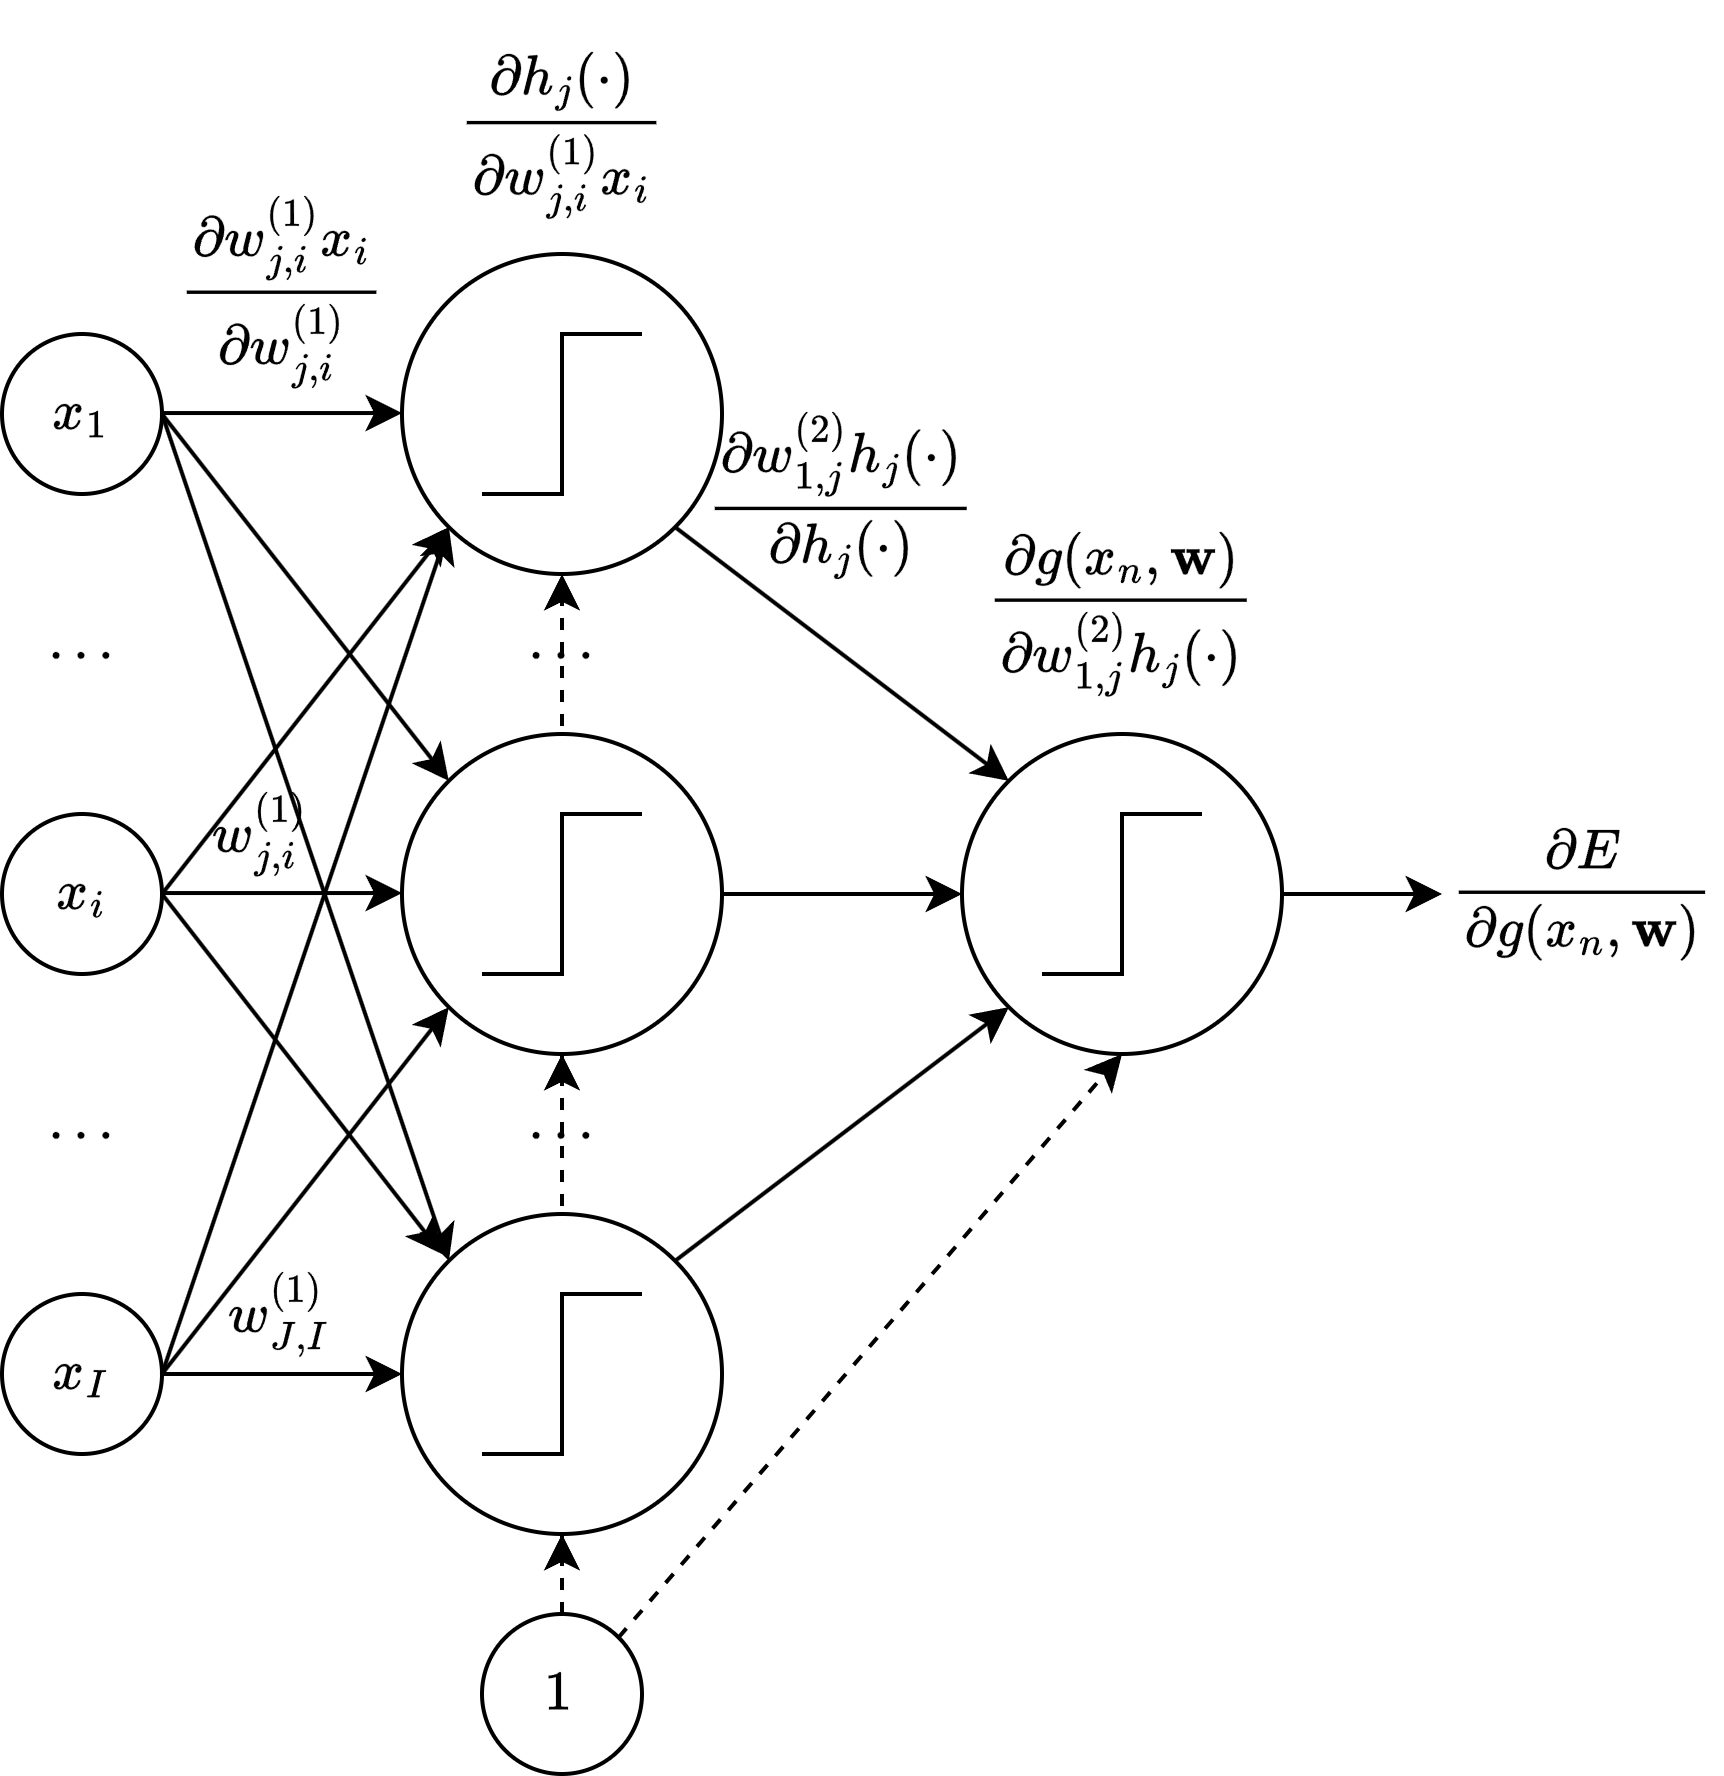
\includegraphics[width=0.75\linewidth]{images/bacfor.png}
    \caption{Forward and backward passes in Neural Networks}
\end{figure}
This approach allows for a systematic and parallelizable way of calculating the gradient, minimizing the computation needed for each update and ensuring that the network can be trained efficiently.

\subsection{Batch normalization}
To achieve faster convergence in neural networks, it is beneficial for the inputs to be whitened, meaning they should have a zero mean and unit variance while also being uncorrelated. 
This practice helps mitigate covariate shift. 
However, in addition to external covariate shifts, networks can experience internal covariate shifts, where the distribution of each layer's inputs changes during training.
Batch normalization is a powerful technique to address this issue.

Batch normalization normalizes the activations of each layer, forcing them to take on values that approximate a unit Gaussian distribution at the start of training. 
It is typically implemented as follows:
\begin{itemize}
    \item A BatchNorm layer is added after fully connected or convolutional layers and before the activation functions (nonlinearities).
    \item This layer effectively acts as a preprocessing step at each level of the network but is integrated in a differentiable manner, allowing for backpropagation.
\end{itemize}

\paragraph*{Algorithm}
The input comprises values of $x$ over a mini-batch $\mathcal{B} = \{ x_1, \dots, x_m \}$. 
The outputs are the parameter to be learned $\gamma, \beta$ with respect to the given min-batch.
\begin{algorithm}
    \caption{Batch normalization}
    \begin{algorithmic}[1]
        \State Compute mini-batch mean: $\mu_{\mathcal{B}} \gets \frac{1}{m} \sum_{i=1}^m x_i$
        \State Compute mini-batch variance: $\sigma_{\mathcal{B}}^2 \gets \frac{1}{m} \sum_{i=1}^m (x_i - \mu_{\mathcal{B}})^2$
        \State Normalize: $\hat{x}_i \gets \frac{x_i - \mu_{\mathcal{B}}}{\sqrt{\sigma_{\mathcal{B}}^2 + \epsilon}}$     
        \State Scale and shift: $y_i \gets \gamma \hat{x}_i + \beta$
    \end{algorithmic}
\end{algorithm}
Batch normalization has several notable benefits:
\begin{itemize}
    \item \textit{Improved gradient flow}: it enhances the flow of gradients through the network, making it easier to train deep architectures.
    \item \textit{Higher learning rates}: allows for the use of higher learning rates, leading to faster convergence.
    \item \textit{Reduced dependency on weight initialization}: the strong dependence on initial weights is mitigated, as the normalization process stabilizes the learning.
    \item \textit{Regularization effect}: acts as a form of regularization, slightly decreasing the need for techniques like dropout.
\end{itemize}
By incorporating batch normalization into neural network architectures, practitioners can significantly enhance training efficiency and model performance.

\subsection{Weight initialization}
The effectiveness of gradient descent in neural networks is highly dependent on how weights are initialized at the start. 
Various approaches to weight initialization can significantly impact the convergence speed and stability of the network: 
\begin{itemize}
    \item \textit{Zero initialization}: setting all weights to zero is ineffective because it results in zero gradients, meaning no learning occurs. 
        Symmetry is never broken, and the model fails to converge.
    \item \textit{Large weights}: Initializing with large weights is also problematic. 
        In deep networks, large initial weights can cause gradients to explode as they propagate back through the layers, leading to instability and slow convergence.
    \item \textit{Small weights} (Gaussian distribution): initializing weights with small values from a Gaussian distribution, such as $\mathbf{w}\sim \mathcal{N}(0,\sigma^2)=0.01$, works for shallow networks but may pose challenges for deeper architectures. 
        Small initial weights in deep networks can cause the gradients to shrink as they pass through each layer, slowing down learning and potentially leading to the vanishing gradient problem.
\end{itemize}
In deep networks, weight initialization plays a critical role in avoiding the vanishing or exploding gradient problems:
\begin{itemize}
    \item \textit{Small weights}: if the initial weights are too small, gradients shrink during backpropagation, eventually becoming so small that learning effectively halts.
    \item \textit{Large weights}: if the initial weights are too large, gradients can grow excessively, leading to unstable learning or divergence.
\end{itemize}
To address these issues, specific initialization methods have been proposed to ensure that the gradients remain balanced as they propagate through the network.

\paragraph*{Xavier initialization}
Xavier initialization, proposed by Glorot and Bengio, aims to maintain the variance of the activations across layers, ensuring that signals neither vanish nor explode.
Suppose we have an input vector $\mathbf{x}$ with $I$ components, and a linear neuron with random weights $\mathbf{w}$. 
The output of the neuron is:
\[h_j=w_{j,1}x_1+\dots+w_{j,i}x_i+\dots+w_{j,I}x_I\]
The variance of each term $w_{j,i}x_i$ is:
\[\text{Var}(w_{j,i}x_i)=\text{Var}(w_{j,i})\text{Var}(x_i)\]
Assuming $x_i$ and $w_i$ are independent and identically distributed , the variance of the output $h_j$ becomes:
\[\text{Var}(h_j)=I\times\text{Var}(w_i)\text{Var}(x_i)\]
To keep the variance of the output the same as the input, Xavier initialization sets the weights as:
\[\mathbf{w}\sim \mathcal{N}\left(0,\frac{1}{n_{\text{in}}}\right)\]
Here, $n_{\text{in}}$ is the number of input units to the neuron.
For the gradients, Glorot and Bengio derived that the variance of the weights should also consider the number of output units $n_{\text{out}}$, leading to the refined initialization:
\[\mathbf{w}\sim \mathcal{N}\left(0,\frac{2}{n_{\text{in}}+n_{\text{out}}}\right)\]
This approach works well for activation functions like sigmoid or hyperbolic tangent.

\paragraph*{He initialization}
More recently, He initialization was proposed specifically for networks using ReLU activations. 
Since ReLU activation functions only pass positive values, He initialization sets a slightly larger variance to prevent shrinking gradients. 
It uses the following distribution:
\[\mathbf{w}\sim \mathcal{N}\left(0,\frac{2}{n_{\text{in}}}\right)\]
This method helps maintain better gradient flow, especially in deep networks with ReLU activations, and is widely adopted in modern architectures.